\chapter{文獻探討}


\section{品牌聲望}

一、品牌的定義

美國行銷學會(American Medical Association,AMA)
對品牌的定義為:名稱 (Name)詞語(Term) 標記(Sign)象徵(Symbol )設計(design)


\section{品牌知覺}
Aaker (1990) 將消費者對品牌的知覺品質定義為消費者對於某一 項品牌產品整體品質的認知(水)準,或消費者對在(特)定目的下相對於其他品牌, 對某品牌產品或服務全面品質的主觀滿意程度。

kelle(1993)認為品牌認知是指在消費者記憶中較強的品牌聯想與連接。Aacker(1991)認為,

Dawar and Parker(1994) 指出消費者挑選產品以品牌聲望為主要考量
Herbig and Milewica(1996) 正向的品牌聲望有助收益增加。
Kowallczyk and Pawlish(2002)公司聲望是影響消費者購買的因屬之一。
Veloutsou and Moutinho(2009)維持和提升公司聲望比強化消費者滿意度更重要
Priporas and Kamenidou(2011)品牌聲望佈警示品牌保證,也是行銷推廣的利器
\section{品牌行銷}

keller (1998)提出可以從四種角度說明品牌的意義與功能\cite{Aaker}

1.品牌可以用圖案來辨別,可用來與競爭者來區別

2.品牌一致的保證與承諾,是消費者在購買或使用之前的感覺產品的價值與品質

3.品牌是可以自我投射形象,品牌個性的傳達

4.品牌是一組是有關產品的定位,代表一致性品質與功能性的集合,可作為消費者決策購買時的線索

Aaker (1996) 認為品牌權益可分為:(1)品牌知名度 (Brand Awareness)、(2)品牌忠誠度 (Brand loyalty) 、(3)品牌知覺品質 (Brand perceived quality) 、(4)品牌聯想 (Brand Association)、(5)其他品牌專屬資產 (Brand Speciality Asset) 。
    Keller (1998)亦詳細地指出,品牌權益實包含:(1)品牌鮮明度 (Brand Salience):可能會影響消費的判別難易度,(2)品牌績效 (Brand Performance):可以滿足消費者所需功能,(3)品牌形象 (Brand Image):在消費者心中產生對品牌抽象整體概念,(4)品牌判斷 (Brand Judgment) :消費者對於品牌理性層面的判定,(5)品牌情感 (Brand Feeling):消費者對品牌情感的概念與特性,或是社會認可的特徵,(6)品牌共鳴 (Brand Resonance):與消費者品牌關係的最高層次,是由品牌情感到具體行動購買的具體表現,例如主動參與及重複購買的行為忠誠度。

\begin{figure}[htbp]
\centering 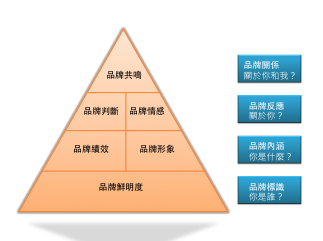
\includegraphics[%
  width=13cm,keepaspectratio]{images/keller2008}
\caption{\label{fig:keller}來自keller2008}
%(資料來源:本研究整理)
\end{figure}


\section{消費者行為}
早期的消費者行為通常都以消費者動機來當研究核心,隨著各位學者長年研究下來提出了許多相關理論的模式,但是現在研究後期主要都已決策的過程為主要核心


%如圖整理~\ref{fig:Consumer1}

%如圖整理~\ref{fig:Consumer2}

\begin{figure}[htbp]
\centering 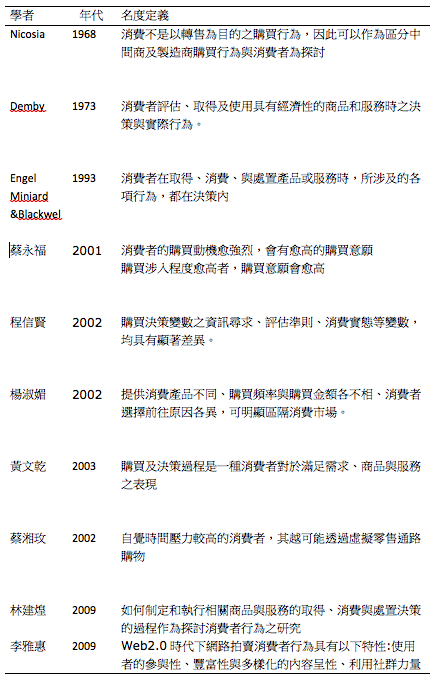
\includegraphics[%
  width=13cm,keepaspectratio]{images/Consumer1}
\caption{\label{fig:Consumer1}本研究整理}
%(資料來源:本研究整理)
\end{figure}

\begin{figure}[htbp]
\centering 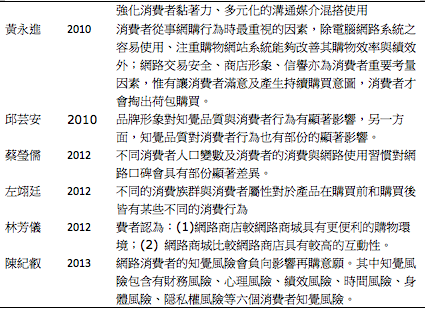
\includegraphics[%
  width=13cm,keepaspectratio]{images/Consumer2}
\caption{\label{fig:Consumer2}本研究整理}
%(資料來源:本研究整理)
\end{figure}



\section{消費者行為理論(Consumer Behavior Theory)}
\subsection{消費者行為定義}
消費者
\begin{figure}[htbp]
\centering 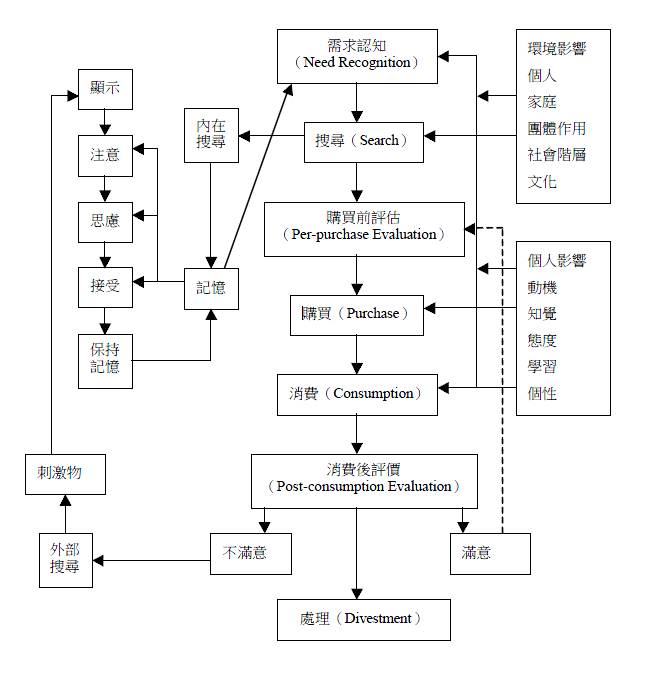
\includegraphics[%
  width=13cm,keepaspectratio]{images/ConsumerBehaviorTheory}
\caption{\label{fig:ConsumerBehaviorTheory}RogerD. Blackwel、PaulW.Miaiard、JamesF.Engel ,CONSUMER  BEHAVIOR,Harcout College Publishers,P38}
%(資料來源:本研究整理)
\end{figure}

\subsection{購買意願之購買決策過程}
Engel, et al (2001) 認為,消費者決策過程的五個重要階段如圖~\ref{fig:Engel}

1.問題認知

購物過程開始時於消費者觀察自身需求與問題來源的認知 ;消費者在問題認知方面會受到外在因素影響(文化,人口統計變數,慘考群體)與個人因刺激,引起消費者產生動機

2.尋求

消費者在確定自己本身所需後,會根據自身問題或是所需來尋求相關資訊,以進行購物決策。一般的消費者收集資訊通常都分為兩種來源,內部搜尋與外部搜尋;消費者,通常會先從自身的記憶中搜尋所需的相關資訊,如過記憶中沒有相關記憶就會改以外部搜尋,獲得協助決策的相關資訊,外部搜尋的資訊如:家人,朋友,廣告,網路等。
           
3.方案評估

搜尋資料完後,就可以對所需要的選著方案做評估與最後的決策。通常消費者都是夠過各項評估的標準與尺度來評定購買的方案。

4.選擇

經過以上敘述方案評估過程後,消費者會以全部方案中選擇最適合的方案,並購買的行動。

5.結果 

當消費者購買產品後,因為本身對產品的期望結果與實際使用的結果,兩種之間的感覺受差異。
一般消費者購買的商品使用後心裡的感受主要有三中結果

符合期望:消費者使用購買的產品後的結果表現符合預期的期望,沒有特別好或壞的感覺

非常滿意:消費者使用購買的產品後的結果表現超過預期的期望,導致心裡的感覺很滿意

不滿意:消費者使用購買的產品後的結果表現低於預期的期望,導致心裡的感覺很不滿意的反應

\begin{figure}[htbp]
\centering 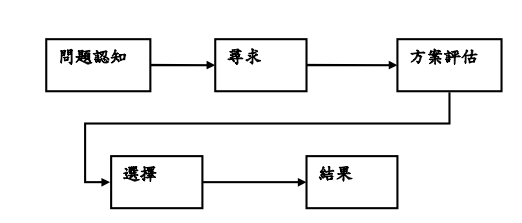
\includegraphics[%
  width=13cm,keepaspectratio]{images/Engel}
\caption{\label{fig:Engel}Engel, et al (2001)}
%(資料來源:本研究整理)
\end{figure}

\subsection{消費者行為理論介紹}

\section{La jolla樂活雅}

公司簡介:

經營據點:台灣:台北市大安區光復南路446號七樓 
               美國:2231 N. 23rd St. Beaumont, TX 77706

 經營理念:富紳國際實業有限公司主要從事首飾及貴金屬零售業;擁有為數不少的客戶群。
最初,是由兩位業餘華裔設計師,自行創作手工珠寶藝品,由於設計風格獨特,大受消費者的歡迎及喜愛,總是供不應求。設計師們有鑑於手工飾品無法大量生產,又觀察到,在未來的飾品趨勢中,鈦飾品將取代金銀等貴重金屬,成為高級珠寶設計重要材質,因此決定發展鈦鍺飾品。

以生產設計鈦鍺精品為主的富紳國際,也接受客戶OEM及ODM訂單。舉凡項鍊、手鍊、戒指、袖扣等商品,並供貨給日本、美國等客戶及珠寶精品業者。
另外,富紳國際亦提供客製化服務,承接結合鈦飾品及頂級鑽石之客製化訂單,為消費者
提供獨一無二的商品訂製服務。

發展至今,富紳國際已擁有自己的設計師及協力生產工廠,從來圖打樣、來樣製作及專業生產一應俱全。專屬設計師群發揮豐富的創造力,賦與每一款設計精品獨創的理念,再結合老師傅精湛的珠寶鑲工技藝,精心打造每一分一毫細微處,提供國內外客戶最與眾不同、匠心獨具的頂級鈦鍺珠寶精品。

 企業文化:La Jolla品牌概念來自於美國加州。 La Jolla,源於西班牙文「珠寶」之意-「聖地牙哥的海洋之珠」,因為是西班牙文,所以唸法獨特,J的發音為H的氣音,唸作[ la-ho-ya](接近中文發音”拉荷亞)。La Jolla是一個位於美國加州San Diego的明媚小鎮。

在「陽光.沙灘.美麗海岸」的見證下,品牌創辦人遇見了”命中注定”的另一半,並於 La Jolla
小鎮買下了別具意義的定情戒,兩人互許真愛,相守一生。這份難能可貴的愛情,讓他們
決心將這份浪漫,轉化為璀燦迷人的健康概念純鈦飾品,將他們勇於追尋真愛的故事,透
過La Jolla精品,不斷的傳遞出去。

La Jolla品牌理念-Pure and  Trendy

Pure 材質純度嚴選 

Trendy 引領現代時尚精品風格 

「 La Jolla期許能結合藝術、自然、愜意美好的一切事物,以獨到細膩的品味設計、純鈦
的材質,帶來對生命最美好的感動。」 有別於一般市售的大眾化純鈦飾品, La Jolla
品牌創辦人堅持自我品味,精心打造一個具有現代時尚個性的純鈦精品。旗下專業設計師
更以獨創的設計理念,賦與每款飾品生命力,並結合老師傅細緻的鑲工手藝,極致講究每
一分每一毫細微的作工,呈現出純鈦精品的高雅質感及活力,演繹品味獨具的 La Jolla
純鈦精品新魅力。
                                                                                      
                             by品牌創辦人CORA LIU
(資料來源:La Jolla 樂活雅鈦鍺精品)
 
品牌故事

有別於一般市售的大眾化鈦鍺飾品,La Jolla品牌創辦人CORA LIU堅持自我品味,精心打造一個具有現代時尚個性的鈦鍺精品。旗下專業設計師更以獨創的設計理念,賦與每款飾品生命力,並結合老師傅細緻的鑲工手藝,極致講究每一分每一毫細微的作工,呈現出鈦鍺飾品的高雅質感及活力,演繹品味獨具的La Jolla鈦鍺精品新魅力。

\begin{figure}[htbp]
\centering 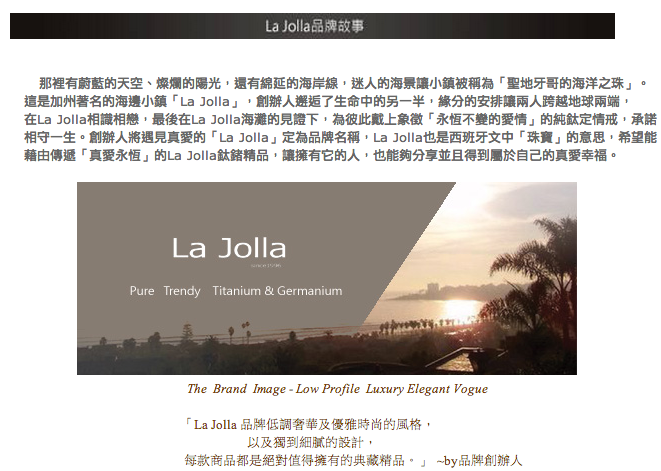
\includegraphics[%
  width=13cm,keepaspectratio]{images/LaJolla}
\caption{\label{fig:LaJolla}LaJolla樂活雅鈦鍺精品}
%(資料來源:本研究整理)
\end{figure}


